In the experimental evaluation part, we address the following 
research questions:
\begin{itemize}
\setlength{\itemsep}{0pt}
\item {\textbf{RQ1:} Can \prototype discover more deeper bugs?}
\item {\textbf{RQ2:} Can distance based seed selection method 
	improve performance of path discovery?}
\item {\textbf{RQ3:} How does each component contribute to 
	path discovery?}
\end{itemize}

More specifically, RQ1 investigates the bug discovery ability of 
\prototype and compares the results with other vulnerability 
detection tools including fuzz testing and dynamic symbolic execution. 
RQ2 evaluates our distance based seed selection on several 
real-world programs to see whether our method can discover more 
unique paths than the state-of-the-art fuzzer: AFL. RQ3 evaluates 
the unique path discovery performance of \prototype and 
investigates the performance contribution of each isolated 
component (i.e. \textit{SPF} and \textit{Searcher}).

%TODO: experimental setups, including the OS, RAM, and CPUs.

\subsection{Vulnerability Detection (RQ1)}
We evaluated the bug discovery ability of our method with two 
different benchmarks and some real world software. The first 
benchmark is a demo program which is named as \emph{CommonMB}. 
The second benchmark is \emph{LAVA}, which was released in 2016 
to test different vulnerability discovery tools \cite{dolan2016lava}. 
In the following sections, we are going to introduce the 
two benchmarks, and discuss the testing results of \prototype
as well as other off-the-shelf vulnerability discovery tools 
(LibFuzzer \cite{libfuzzer}, AFL, KLEE, S2E, Driller, and VUzzer) in detail.

\subsubsection{CommonMB}
\noindent The \emph{CommonMB} benchmark is a demo program which contains 
9 different memory error bugs. These bugs can be triggered only when 
feeding the program with specifically crafted input. There are four 
different kinds of functions in this benchmark, i.e., 2 compare-style 
functions, 3 math-style functions, 2 checksum-style functions and 2 
logic-style functions. The compare functions contains bugs that can 
only be triggered when the values of specific parts of the input equal 
to specific constant immediate numbers; the bugs in math functions 
can be triggered when the results of math operation on some specific 
parts of the input equal to specific constant immediate numbers; the 
checksum related bugs can only be triggered when the input data 
successfully goes through the checksum checking points; and the logic 
bugs utilize two simple logical games (maze and semi-sudoku) as the 
constraints for triggering the bugs, which means the bugs can only be 
triggered when the testing engine successfully solves the games.

The bugs in \emph{CommonMB} benchmark represent the common bug conditions 
in real-world programs. For example, compare-style bugs denote the bugs 
that depend on some specific/interesting values in the program; 
checksum-style bugs stands for the bugs whose inputs are well-formatted, 
such as PNG file.
So evaluating a vulnerability detection tool on such a benchmark can 
reflect its ability of discovering bugs in real world programs.

Table~\ref{CommonMB-results-detail} shows the overall results of 
different vulnerability discovery tools as well as \prototype 
with same test environment (10 cores and 12 hours).
% Explain the result like that cmp-style vulnerabiities are easy to find
We can see that all these tools have successfully triggered the 
two compare-style bugs (i.e., \textit{cmp16} and \textit{cmp32}). 
This is because there two functions are in the shallow surface of 
this benchmark and the conditions to trigger the bugs are simpler 
than the others.  

% Explain the result, for example, why add32 cannot be found by KLEE...
Fuzz testing tools discovered few math-bugs than symbolic execution 
tools in average.
For example, AFL discovered the \textit{add16} and LibFuzzer triggered 
one more bug (i.e., \textit{add32}). And these two fuzzer both failed 
to uncover the bug that guarded by complex mathematic operations. 
All tools that leverage symbolic execution except KLEE successfully 
triggered all these three bugs since symbolic execution is good at 
solving such corner cases. One interesting point in this table is that 
KLEE failed to trigger \textit{add32} and \textit{complex} bugs. 
This is because KLEE forks too many states in checksum functions 
which raise the serious ``state explosion'' problem. 

S2E provides function models for basic functions that may fork too 
many states, like \texttt{strcpy}, \texttt{strcat}, \texttt{crc16},
 and \texttt{crc32}. Based on these models, S2E and \prototype 
 discovered the two bugs that related to checksum successfully 
 (note that this does not mean S2E can break these checksum functions). 

Logic-style vulnerabilities are difficult for all tools to uncover 
because the number of states will be infinite in the worse case.
For example, when solving a maze, the possible oscillation between 
two opposite steps (such as step forward and step backward) 
will stop the engine from finding new paths.
With the help of our seed selection method, \prototype selected 
the seed file with the maximum average distance to schedule. 
Since this distance metric tries to maximize the memory coverage, 
\prototype successfully triggered the bug after covering all 
the memory access to the maze array. 
% Explain why the sudodu is so hard to touch
However, our \prototype failed to trigger the bug in \textit{sudoku}. 
This is because different seed files of the \textit{sudoku} have no 
significant differences (i.e., no more code/branch and memory coverage), 
which confuses our seed selection method.

\begin{table*}[!t]
\processtable{Evaluation results on \textit{CommonMB} in detail.
	\label{CommonMB-results-detail}}
{\begin{tabular*}{20pc}{ccccccccccc}\toprule
	& \multicolumn{2}{c}{CMP}  & \multicolumn{3}{c}{MATH} & \multicolumn{2}{c}{CHECKSUM} 
	& 	\multicolumn{2}{c}{LOGIC} & \\ 
	    Tool & cmp16 & cmp32 & add16 & add32 & complex & crc16 & 
	    crc32 & maze & sudoku & Total Crashes (\#) \\
\midrule
		AFL 		& Y & Y & Y & N & N & N & N & N & N & 3 \\
		LibFuzzer	& Y & Y & Y & Y & N & N & N & N & N & 4\\
		KLEE		& Y & Y & Y & N & N & N & N & N & N & 3\\
		S2E			& Y & Y & Y & Y & Y & Y & Y & N & N & 7\\
		Driller		& Y & Y & Y & Y & Y & N & N & N & N & 5\\
		\prototype	& Y & Y & Y & Y & Y & Y & Y & Y & N & 8\\
\botrule
\end{tabular*}}{}
\end{table*}

\subsubsection{LAVA Benchmark}
In 2016, Dolan-Gavitt et.al. developed a technique, namely LAVA, to 
automatically inject secure-related bugs into some Linux utilities for 
evaluating the bug-finding tools \cite{dolan2016lava}. These bugs are 
all hard-to-reach memory errors. In the paper of LAVA, the authors describe 
their results on the evaluation of coverage based fuzz testing, an SAT-based 
approach on the benchmark. The LAVA benchmark has two corpus sets, 
i.e., \textit{LAVA-1} and \textit{LAVA-M}.

\textit{LAVA-1} injected 69 different bugs into the \texttt{file} program 
in Linux CoreUtils. There are two types of buffer overflow vulnerabilities 
were injected, one is \emph{Range} and the other one is 
\emph{Knob-and-trigger (KT)}. The Range style bugs are triggered if the 
magic value is in some range and also check the value to determine how much 
to overflow. And in the KT bug, two bytes in the input are checked against 
a magic value to determine if the overflow will happen and another two bytes 
determine how much to overflow. Both the two types of bugs were designed to 
mirror real bug patterns which can be used to evaluate the ability of 
bug-finding tools. Compared \textit{LAVA-1}, which injected only one bug 
in the program, \textit{LAVA-M} injected more than one bug into four 
different programs in CoreUtils that took file input: \texttt{base64}, 
\texttt{md5sum}, \texttt{uniq}, and \texttt{who}, so \textit{LAVA-M} is a 
better benchmark to evaluate the vulnerability discovery tools that are 
designed to work for a long time on programs that may contain multiple bugs.

\begin{table}[!b]
\processtable{Evaluation results on \textit{LAVA-1}\label{LAVA-1}}
{\begin{tabular*}{20pc}{@{\extracolsep{\fill}}ccccccc@{\extracolsep{\fill}}}\toprule
& $2^0$ & $2^7$  & $2^{14}$ & $2^{21}$ & $2^{28}$ & KT \\
	      Tool   & (12 bugs) & (10 bugs) & (11 bugs) & (14 bugs) & (12 bugs) & (10 bugs)\\
\midrule
		FUZZER 		& 0   & 0   & 1    & 11    & 9     & 2  \\
		SES	        & 1   & 0   & 1    & 3     & 0     & 1  \\
		AFL		    & 0   & 0   & 2    & 10    & 9     & 1   \\
		S2E			& 3   & 2   & 3    & 4     & 3     & 2   \\
		\prototype	& 10  & 10  & 11   & 13    & 11    & 7   \\
\botrule
\end{tabular*}}{}
\end{table}

Table~\ref{LAVA-1} summarized the results of bug finding evaluation on 
\textit{LAVA-1} from the LAVA paper as well as some popular off-the-shelf 
tools (AFL and S2E). The maximum testing time for each bug was five hours. 
From this table, we can see that the \textbf{FUZZER} and \textbf{SES} 
mentioned in the paper only found 23 bugs and 6 bugs respectively in total. 
AFL found fewer paths than S2E in the small ranges ($2^0$, $2^7$ and $2^{14}$) 
but it outperformed S2E in larger ranges. 

\prototype discovered 62 bugs which was much more than the FUZZER and the 
SES tools separately. In particular, we triggered all the bugs in $2^7$ and 
$2^{14}$ ranges. And also found most of the KT bugs (70\%) which cannot be 
touched effectively by the FUZZER and SES tools. 

Table~\ref{LAVA-M} describes the evaluation results on LAVA-M of the FUZZER 
and SES which are mentioned in the LAVA paper. We also listed the results 
of VUzzer and \prototype in this table. 
\begin{table}[!b]
\processtable{Evaluation results on \textit{LAVA-M}\label{LAVA-M}}
{\begin{tabular*}{20pc}{@{\extracolsep{\fill}}cccccc@{}}\toprule
	     & \texttt{base64} & \texttt{md5sum} & \texttt{uniq} & \texttt{who} &   \\
	     Tool    & (44 bugs) & (57 bugs) & (28 bugs) & (2136 bugs) &  Total\\
\midrule
		FUZZER 		& 7  & 2  & 7    & 0   & 16  \\
		SES	        & 9  & 0  & 0    & 18  & 27  \\
		VUzzer		& 17 & 1* & 27   & 50  & 95 \\
		\prototype	& 37 & 29 & 28   & 203 & 297 \\
\botrule
\end{tabular*}}{}
\end{table}


As mentioned in the LAVA paper, SES cannot find any bugs in \texttt{uniq} and 
\texttt{md5sum}. And the reasons are the control flow is too unconstrained in 
\texttt{uniq} and SES failed to execute any code past the first instance of 
the hash function. Because our symbolic execution is driven by a concrete seed 
input, these two problems will be eased to a large extent, leading to the 
discovery of more bugs. Particularly, for program \texttt{md5sum}, VUzzer can 
only trigger one bug because it fails to get through the first crash to parse 
more of any input, whereas \prototype successfully triggered 29 bugs in 
\texttt{md5sum}.

\subsubsection{Real-World Programs}
We selected several real world programs to evaluate the ability of unknown bug 
discovery of our system. The input types of this dataset cover ELF binary, 
multi-media, image, and packet capture. In order to demonstrate the efficiency 
of our system, we also compared our results with AFL and VUzzer. We ran each
 program under the same testing environment with one fuzzing node for 24 hours. 

Table~\ref{zero-days} shows the results of our testing. 
From the table we can see that during 24 hours, \prototype triggered 403 
unique crashes in the dataset which outperformed vanilla AFL (181 unique crashes) 
and VUzzer (192 unique crashes). 
We can also derive from this table that our method gains little for \texttt{mp3gain} 
and \texttt{madplay}. This is because our symbolic execution engine does not support 
the float number operation when handing MPEG/WAV format (for example, all the 
writing operation to \texttt{XMM} registers will be concretized). This concretization 
lost some interesting paths and made less contribution to bug finding(only 2 more 
bugs for \texttt{mp3gain} and 1 more bug for \texttt{madplay}). 
This also explains the phenomena that VUzzer found more bugs in \texttt{mp3gain} 
than \prototype. 
It is interesting that AFL detected 15 more bugs in \texttt{elfparser} than VUzzer. 
This is because the fork server method leveraged in AFL enables the fuzzer can 
execute 51.6x more test cases than VUzzer in the same time, which can also increase 
the probability of finding bugs.

\begin{table*}[!t]
\processtable{Performance of our method VS. AFL \& VUzzer on unknown crashes.\label{zero-days}}
{\begin{tabular}{lccccccc}\toprule
	& & \multicolumn{2}{c}{\prototype} & \multicolumn{2}{c}{AFL} & \multicolumn{2}{c}{VUzzer}\\
		    Program & Input Type & Crashes (\#) & Executed (\#)& 
		    Crashes (\#) & Executed  (\#) & Crashes (\#) & Executed (\#) \\
\midrule
\texttt{elfparser}  & ELF	& 60 &   1.1M & 48   & 1.0M   & 33 & 19.0K    \\
		\texttt{distorm}    & ELF    & 13 &   16.2M   & 0   & 15.7M    & 3 & 93.1K    \\
		\texttt{mp3gain}*   & MPEG	& 43 &   11.3M  & 41  &  11.7M   & 46 &  79.3K  \\
		\texttt{madplay}*   & WAV	& 55 &   15.9M  & 54  & 14.3M    & 52 & 88.7K   \\
		\texttt{optipng}    & PNG    & 49 &   9.5M & 15  &  10.1M   & 32 & 54.1K   \\
		\texttt{tstat}      & PCAP   & 183&   6.4M & 23 &  6.2M   & 26 & 48.5K   \\
		\midrule
		Total      &        & 403   &  & 181 &  & 192 &\\
\botrule
\end{tabular}}{}
\end{table*}

\subsection{Coverage Performance (RQ2)}\label{sec:RQ2}
Our benchmark for coverage performance evaluation consists of 8 real-world binary 
programs, and the input file formats of our benchmark cover a range of types such 
as executables, images, archives and network packets.

To set the baseline of coverage performance, we utilized the state-of-the-art 
coverage based fuzzer AFL \cite{online:afl} and configured it to run under 
\textit{binary-testing} (i.e., option `-Q' is turned on) mode with one 
single work node.
 We collected and compared \textbf{the number of unique paths} found by 
 AFL and our distance based seed selection method.
 Then we select the most effective distance metric for 
 subsection~\ref{sec:RQ3}.
 All the evaluations lasted for 24 hours.

The evaluation results were shown in Table~\ref{PD-8samples}. We have 
investigated the three distance measures mentioned before (i.e., EU, CS, 
and JI) as well as the original seed selection strategy (Order) from 
vanilla AFL which selects test case in the seed queue one by one.
From this table, we can see that by prioritizing the mutation orders of 
seeds, the fuzzer can touch more unique paths in average.
 More clearly, Figure~\ref{path-detail}(a) shows the normalized unique 
 paths to vanilla AFL (i.e., orderly selection) for these 8 programs 
 based on the results in Table~\ref{PD-8samples}.
\begin{table}[!b]
\processtable{Number of unique paths discoverd for 8 sample programs\label{PD-8samples}}
{\begin{tabular*}{20pc}{@{\extracolsep{\fill}}lrrrr@{}}\toprule
	     Program  & Order\# & EU\# & CS\# & JI\# \\
\midrule
		\texttt{readelf}  &    2753 & 4595 & 5314 & 5062 \\
		 \texttt{djpeg }  &    2802 & 3020 & 4198 & 3390 \\
		\texttt{objdump} &    1755 & 2200 & 2960 & 2133 \\
		 \texttt{gzip }  &    1440 & 1564 & 1754 & 1588 \\
		 \texttt{ffmpeg}  &    5022 & 5993 & 6181 & 5801 \\
		\texttt{tcpdump}  &    3399 & 3673 & 4267 & 2950 \\
		\texttt{capstone} &    5626 & 6008 & 6066 & 5873 \\
		\texttt{gif2png}  &     912 &  981 & 1100 &  997 \\ 
\botrule
\end{tabular*}}{}
\end{table}


From Figure~\ref{path-detail}(a), we can see that both EU and CS metrics 
can outperform vanilla AFL on discovering unique paths for all programs 
in our benchmark. However, the average performance gain of EU is 
lowers than CS metric. 
Compared with the other two distance measures, JI is the most unstable 
strategy which discover more unique paths for some programs, like 
\texttt{readelf}, \texttt{djpeg}, but also brings performance overhead 
for some others, such as \texttt{tcpdump}.

An interesting point from Figure~\ref{path-detail}(a) is that, for 
\texttt{capstone}, the performance gain of CS metric is not as 
significant as the other 7 programs (found only 8\% more paths 
than vanilla AFL).
This is because, in our experiment, the input of \texttt{captone} 
was only plain texture file with some assembly code in it. Such kind 
of input is not as well formatted as other inputs like ELF, JPEG, 
CAP and so on. 
So modifying any parts of the input may have same probability to
 trigger new behaviors which means each seed file in the queue 
 will have nearly the same power to cover new code areas. This 
 also demonstrates that our seed prioritization method will gain 
 more performance for well-formatted inputs.

To demonstrate the path discovery speed along with test time, 
we selected four representative programs, i.e., \texttt{readelf}, 
\texttt{ffmpeg}, \texttt{objdump}, and \texttt{tcpdump}, in our 
benchmark and collected the number of unique paths every two 
hours (the number for each program is normalized to the 
maximum to make this figure more clear).
The results are shown in Figure~\ref{path-detail}(b), where 
the x-axis indicates the test time in hours; while the y-axis 
shows the normalized unique number of paths triggered 
by each strategy.
As shown in Figure~\ref{path-detail}(b), both CS and EU performed 
consistently better than orderly during all the 24 hours.
More specifically, EU performed better than CS in the first 
several hours, and then CS outperformed EU in the following test time.
While JI performed well in \texttt{readelf}, \texttt{ffmpeg} and 
\texttt{objdump}, but it failed to improve the performance in 
\texttt{tcpdump} after testing for 8 hours.
 
Especially for \texttt{ffmpeg}, we can see that in the first 4 hours, 
all of these four selection strategies achieved the same 
performance on discovering unique paths. However, vanilla AFL 
(i.e., Order) failed to trigger more unique paths during 4$\sim$18 
hours before it started to find new paths again.
This is because the mutation areas of seeds that processed 
during 4$\sim$18 hours are overlapped with each other 
(as shown in Figure~\ref{motivate-example}), which will not 
contribute any new paths. However, by selecting seed that has 
longest distance from already explored spaces, our distance based 
seed selection strategy can consistently trigger new paths 
during 24 hours as shown in this figure.

Based on the results, we can obtain that our distance based seed 
selection strategy (especially CS metric) can achieve 
higher performance than vanilla AFL. So we selected CS metric as 
our selection strategy in the following evaluation section.

\begin{figure}[!t]
	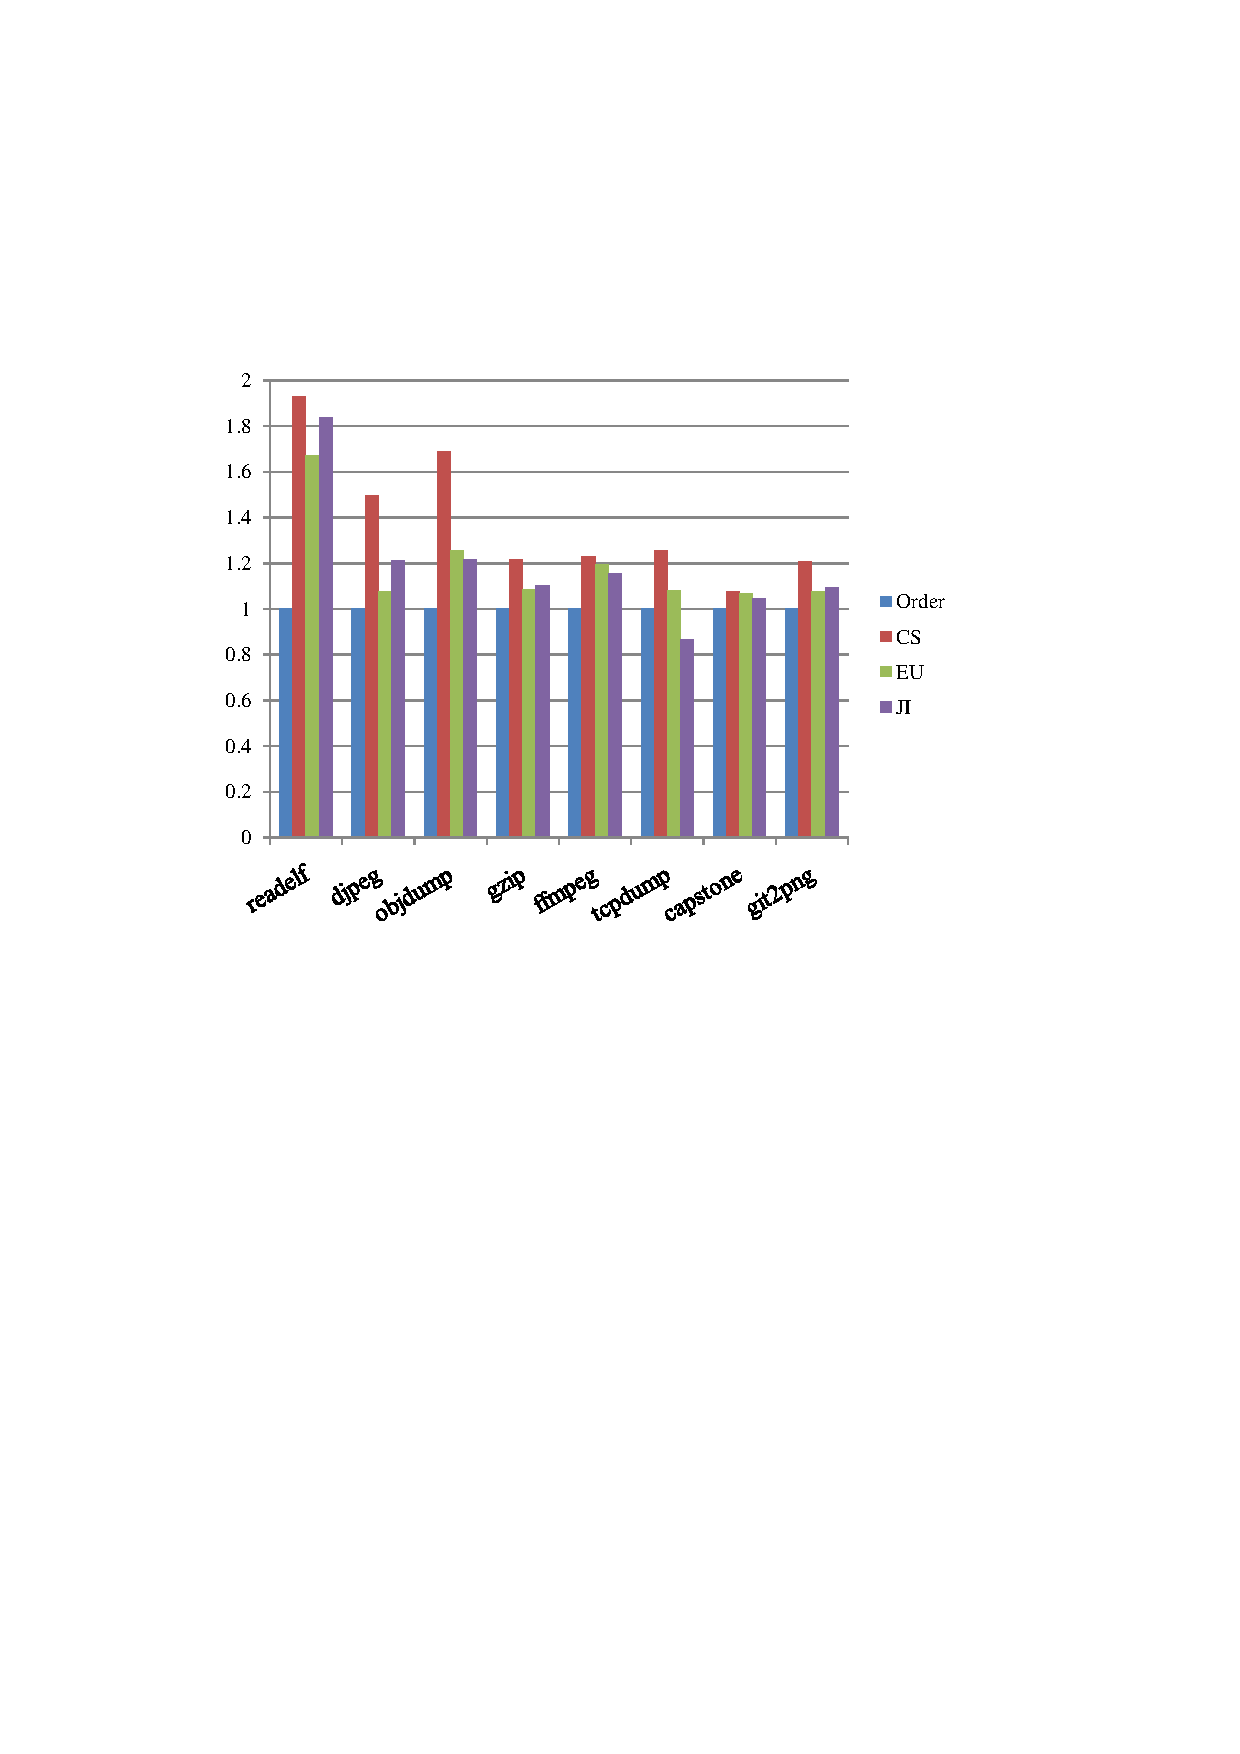
\includegraphics[width=0.45\textwidth, trim={0.2cm 0.4cm 0cm 0cm}, clip]
	{figures/path-discovery.pdf}
	\figfooter{(a)}{Normalized number of unique paths for these 
		four selection strategies to vanilla fuzz testing (i.e., \textit{Order}) }
	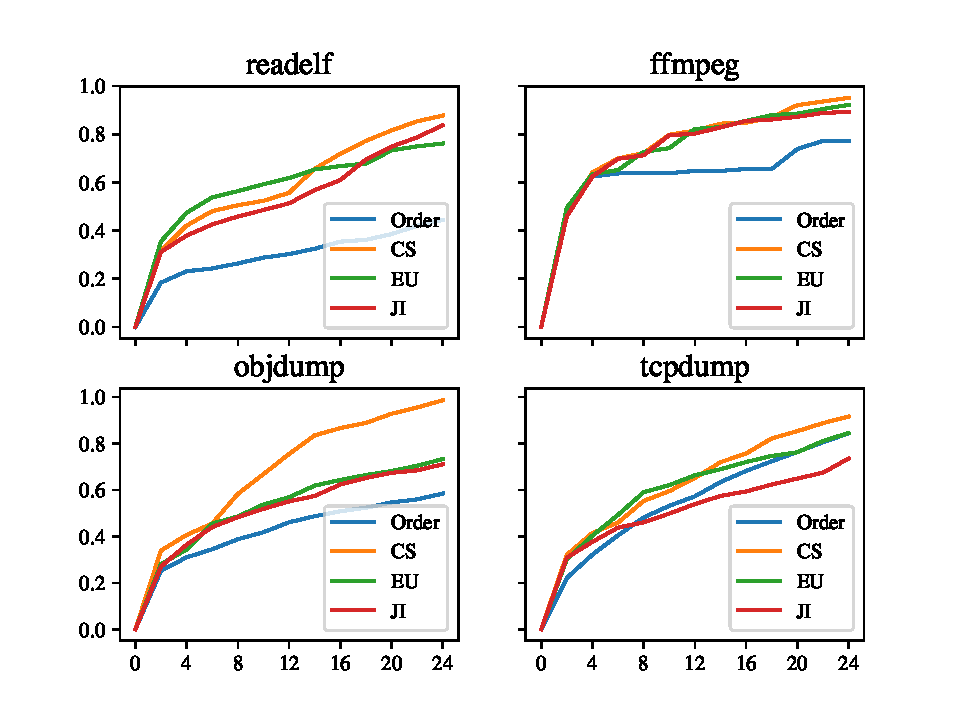
\includegraphics[width=0.45\textwidth, trim={0.15cm 0.1cm 1.5cm 0.8cm}, clip]
	{figures/path-time-detail.pdf} 
	\figfooter{(b)}{Path discovery details along with 24 hours for 
		four sample programs.}\label{fig1}
  \caption{Path discovery results for different seed selection strategies.}
  \label{path-detail}
\end{figure} 

\subsection{Improvement Detail for Each Component (RQ3)} \label{sec:RQ3}
In order to evaluate the contribution of each component on finding 
unique paths, we conducted four experiments (i.e., vanilla AFL fuzz testing, 
symbolic execution assisted hybrid testing (\textit{SEHT}), SEHT with SPF, 
SEHT with SPF\&Searcher) and compared their results in 24 hours.

In our experiments, since Driller \cite{stephens2016driller} does not support 
real-world binary programs very well now (many library functions and system 
calls are not modeled), we reimplemented the mechanism of Driller within 
S2E to collect the results for SEHT. And based on the results of 
subsection~\ref{sec:RQ2}, our searcher employs cosine similarity 
as the distance metric.

Figure~\ref{path-overall-rsults} summarizes the results of how each 
component contribution to the performance improvement. Compared with 
vanilla fuzz testing, symbolic execution assisted hybrid testing can 
discover 11.88\% more unique paths in average. For example, this 
improvement reaches the highest figure of 42.79\% for \texttt{readelf}. 
However, the performance gain is lower than 20\% for the other 7 programs. 
Specifically, \textit{SEHT} triggered only 1.32\% more unique paths 
than vanilla fuzz testing for \texttt{gif2png}. This is because the 
symbolic execution engine does not support to handle float number 
operation. After employing \textit{SPF} which handles symbolic pointers 
and symbolic loops, 7.22\% more unique paths touched by \textit{SEHT with SPF} 
than \textit{SEHT} in average. We can see from this figure that 
the performance of \textit{SEHT} is highly improved by \textit{SPF} 
for \texttt{readelf} and \texttt{objdump} (18.02\% and 22.62\% respectively).
 
This improvement can be continually augmented by cooperating with CS 
searcher (\textit{SEHT with SPF and CS Searcher}). For example, the number 
of unique paths discovered by \textit{SEHT} is increased by 
49.57\% for \texttt{objdump}. In average, the performance of \textit{SEHT} 
is improved by 24.44\% after introducing SPF and CS searcher. From an 
overall viewpoint, \prototype can discover 43.49\% more unique paths 
than vanilla AFL fuzz testing for our benchmark. This improvement is 
because that seeds file with longest distance from already-explored 
spaces have higher likelihood to trigger more fresh branches/paths, 
so solving such seed files earlier by symbolic execution can find more 
fresh seed files than other files. \\

 
Above all, we can obtain that \textit{Searcher} contributes larger 
proportion of contribution to unique path discovery than \textit{SPF}. 
However, this does not mean the contribution of \textit{SPF} is 
negligible. By integrating \textit{SPF} component (i.e., \textit{LCSP} 
and \textit{SLB}), the symbolic execution engine can dive into deeper 
code areas to solve \textit{complex branch conditions} to help fuzzer 
find more fresh paths and discover more hard-to-reach vulnerabilities.

      
\begin{figure}
\begin{center}
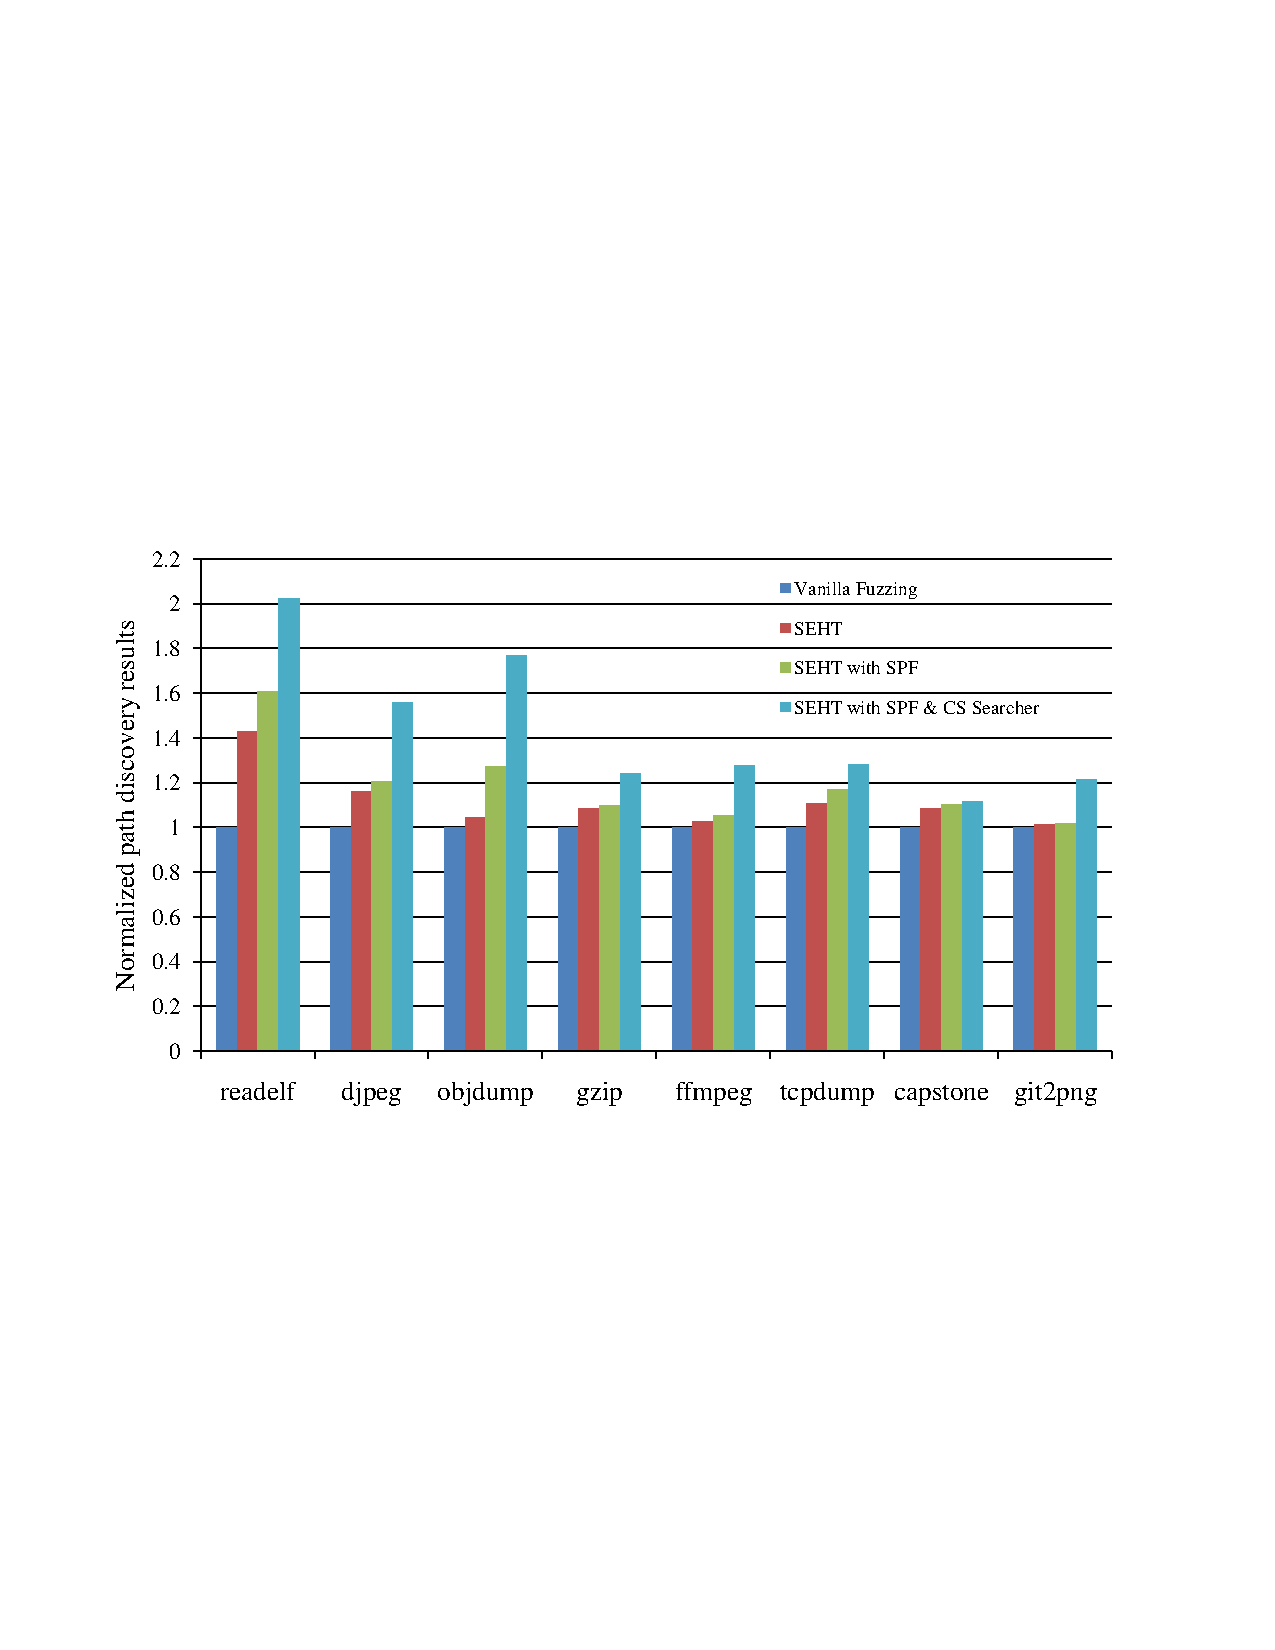
\includegraphics[width=0.5\textwidth]{figures/path-discovery-SPF-CS-all.pdf} 
\caption{Normalized number of unique paths discovered for each component to vanilla fuzz testing.}\label{path-overall-rsults}
\end{center}
\end{figure}